\documentclass{article}

\usepackage{graphicx}
\usepackage[inline]{enumitem}
\usepackage{amssymb}

\providecommand{\sin}{} \renewcommand{\sin}{\mathrm{sen}\hspace{1pt}}
\providecommand{\tan}{} \renewcommand{\tan}{\mathrm{tg}\hspace{1pt}}

\begin{document}
\noindent{}\rule{\textwidth}{0.4pt}
\begin{center}
	C\'alculo 2\\
	Lista 1 --- Integrais \\
	\vspace{0.2cm}
	Prof. Adriano Barbosa
\end{center}
\noindent{}\rule{\textwidth}{0.4pt}

\begin{enumerate}
%%%%%%%%%%%%%%%%%%%%%%%%%%%%%%%%%%%%%%%%%%%%%
\item
\begin{enumerate}[label=\alph*.]
	\item Estime a \'area sob o gr\'afico $f(x) = 1 + x^2$ de $x = -1$ at\'e $x = 2$
		usando tr\^es ret\^angulos aproximantes e escolhendo os $c_i$ como
		extremidades direitas. Ent\~ao, aperfei\c{c}oe sua estimativa utilizando seis
		ret\^angulos aproximantes. Esboce a curva e os ret\^angulos aproximantes.
	\item Repita a parte a.\ usando extremidades esquerdas.
	\item Repita a parte a.\ escolhendo os $c_i$ como o ponto m\'edio de cada subintervalo.
	\item A partir de seus esbo\c{c}os das partes a., b., e c., qual parece ser a melhor estimativa?
\end{enumerate}

%%%%%%%%%%%%%%%%%%%%%%%%%%%%%%%%%%%%%%%%%%%%%
\item
\begin{enumerate}[label=\alph*.]
	\item Calcule a soma de Riemann para $f(x) = x^3 - 6x$ tomando como pontos
		amostrais as extremidades direitas e $a = 0$, $b = 3$ e $n = 6$.
	\item Calcule $\int_0^3 x^3 - 6x\ dx$ pela defini\c{c}\~ao.
\end{enumerate}

%%%%%%%%%%%%%%%%%%%%%%%%%%%%%%%%%%%%%%%%%%%%%
\item O gr\'afico de $g$ consiste em duas retas e um semic\'{i}rculo. Use-o para
	calcular cada integral

\begin{enumerate*}[label=\alph*.]
	\item $\displaystyle\int_0^2 g(x)\ dx$\hfill{}
	\item $\displaystyle\int_2^6 g(x)\ dx$\hfill{}
	\item $\displaystyle\int_0^6 g(x)\ dx$
\end{enumerate*}

\begin{figure}[h]
	\centering
	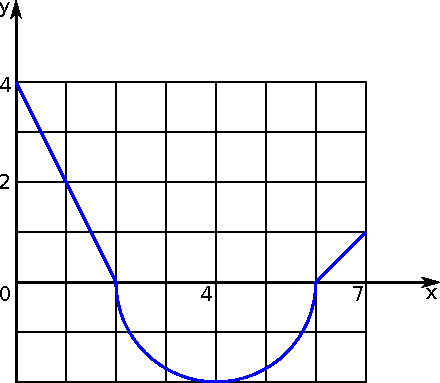
\includegraphics[scale=0.7]{grafico.pdf}
\end{figure}

%%%%%%%%%%%%%%%%%%%%%%%%%%%%%%%%%%%%%%%%%%%%%
\item Calcule as integrais interpretando-as em termos de \'areas.

\begin{enumerate*}[label=\alph*.]
	\item $\displaystyle\int_{-1}^2 1 - x\ dx$
	\item $\displaystyle\int_{-1}^2 |x|\ dx$
\end{enumerate*}

%%%%%%%%%%%%%%%%%%%%%%%%%%%%%%%%%%%%%%%%%%%%%
\item Apenas analisando o gr\'afico das fun\c{c}\~oes, calcule as seguintes integrais

\begin{enumerate*}[label=\alph*.]
	\item $\displaystyle\int_{-1}^1 x\ dx$
	\item $\displaystyle\int_{-1}^1 |t|\ dt$
	\item $\displaystyle\int_{-1}^1 y^2\ dy$
	\item $\displaystyle\int_{-\pi}^{\pi} \sin\theta\ d\theta$
	\item $\displaystyle\int_{-\pi}^{\pi} \cos\phi\ d\phi$
\end{enumerate*}

Deixe os itens b.\ e c.\ em fun\c{c}\~ao de alguma \'area.
	
%%%%%%%%%%%%%%%%%%%%%%%%%%%%%%%%%%%%%%%%%%%%%
\item Use o Teorema Fundamental do C\'alculo para encontrar a derivada das
	fun\c{c}\~oes abaixo

\begin{enumerate}[label=\alph*.]
	\item $\displaystyle g(x) = \int_1^x \frac{1}{t^3 + 1}\ dt$
	\item $\displaystyle G(x) = \int_x^1 \cos(\sqrt{t})\ dt$
	\item $\displaystyle h(x) = \int_{2x}^{3x} \frac{u^2 - 1}{u^2 + 1}\ du$ (dica: use as propriedades de integrais e a regra da cadeia.)
\end{enumerate}

%%%%%%%%%%%%%%%%%%%%%%%%%%%%%%%%%%%%%%%%%%%%%
\item Calcule as integrais

\begin{enumerate}[label=\alph*.]
	\item $\displaystyle\int_1^2 \frac{3}{t^4}\ dt$
	\item $\displaystyle\int_0^{\pi/4} \sec\theta\ \tan\theta\ d\theta$
	\item $\displaystyle\int_{-1}^1 e^{u+1}\ du$
	\item $\displaystyle\int_0^1 x^e + e^x\ dx$
	\item $\displaystyle\int_0^{\pi} f(x)\ dx$, onde $f(x) = \left\{
			\begin{array}{rl}
				\sin x, & \mbox{se } 0 \leqslant x < \frac{\pi}{2} \\
				\cos x, & \mbox{se } \frac{\pi}{2} \leqslant x \leqslant \pi
			\end{array}\right.$
\end{enumerate}

\end{enumerate}

F\'ormulas \'uteis:

$\displaystyle\sum_{i=1}^n i = \frac{n(n+1)}{2}$

$\displaystyle\sum_{i=1}^n i^2 = \frac{n(n+1)(2n+1)}{6}$

$\displaystyle\sum_{i=1}^n i^3 = \left[\frac{n(n+1)}{2}\right]^2$

\end{document}
